\documentclass{beamer}
\usetheme{Madrid}
\usecolortheme{default}

\title{Naive Utility Calculus}
\author{Joseph Low}
\date{August 2025}

\AtBeginSection[]{
  \begin{frame}
  \frametitle{Table of Contents}
  \tableofcontents[currentsection]
  \end{frame}
}

\begin{document}

\frame{\titlepage}

\begin{frame}
\frametitle{Table of Contents}
\tableofcontents
\end{frame}

\section{Introduction}
\begin{frame}
\frametitle{Introduction}
\vfill
\begin{center}
\fcolorbox{blue}{white}{\parbox{0.8\textwidth}{\centering\Large How do we make sense of other people's behavior?}}
\end{center}
\vfill

\pause

\begin{itemize}
    \item<2-> Why did you sleep late last night?
    \pause
    \item<3-> Why did you sign up for this course?
    \pause
    \item<4-> Why did you choose to eat out instead of cooking?
\end{itemize}
\end{frame}

\begin{frame}
\frametitle{Naive Utility}
\begin{center}
\Large $\text{Utility} = \text{Rewards} - \text{Costs}$
\end{center}
\vspace{0.5cm}
\begin{itemize}
    \item There is empirical support that humans intuitively use utility-based reasoning to make sense of other people's behavior
\end{itemize}
\pause

\vspace{0.5cm}
\begin{columns}
\begin{column}{0.5\textwidth}
\begin{center}
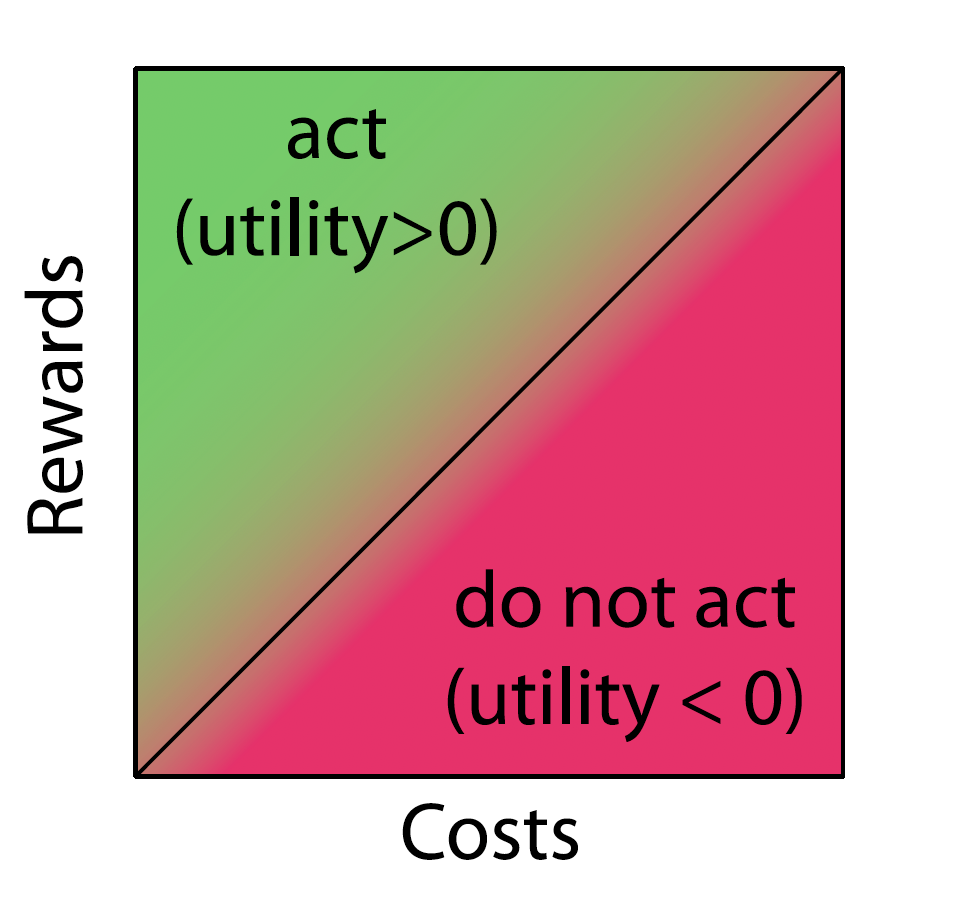
\includegraphics[width=0.8\textwidth]{utility1.png}
\end{center}
\end{column}
\begin{column}{0.5\textwidth}
\pause
\begin{itemize}
    \item Pursue/forego high/low-cost implies reward was even higher/lower
    \pause
    \item Pursue/forego low/high-cost does not give info about reward
\end{itemize}
\end{column}
\end{columns}
\end{frame}

\begin{frame}
\frametitle{Naive Utility Calculus}
\begin{center}
\Large $U(p, o) = R(o) - C(p)$
\end{center}
\vspace{0.5cm}
\begin{itemize}
    \item $U(p, o)$: utility expected from acting according to plan $p$ to reach outcome $o$
    \item $R(o)$: subjective reward the agent expects from outcome $o$
    \item $C(p)$: subjective cost of executing plan $p$
\end{itemize}
\end{frame}

\begin{frame}
\frametitle{Caveats}
\begin{itemize}
    \item \textbf{Descriptive, not normative:} This is not about how people \textit{should} make decisions (economic utility theory)
    \item \textbf{How we actually operate:} This describes how we \textit{intuitively} make sense of other people's behavior
    \item People don't explicitly compute utilities when they act - this is the cognitive framework we use to understand others
\end{itemize}
\end{frame}

\begin{frame}
\frametitle{Utility and Efficiency}
\begin{center}
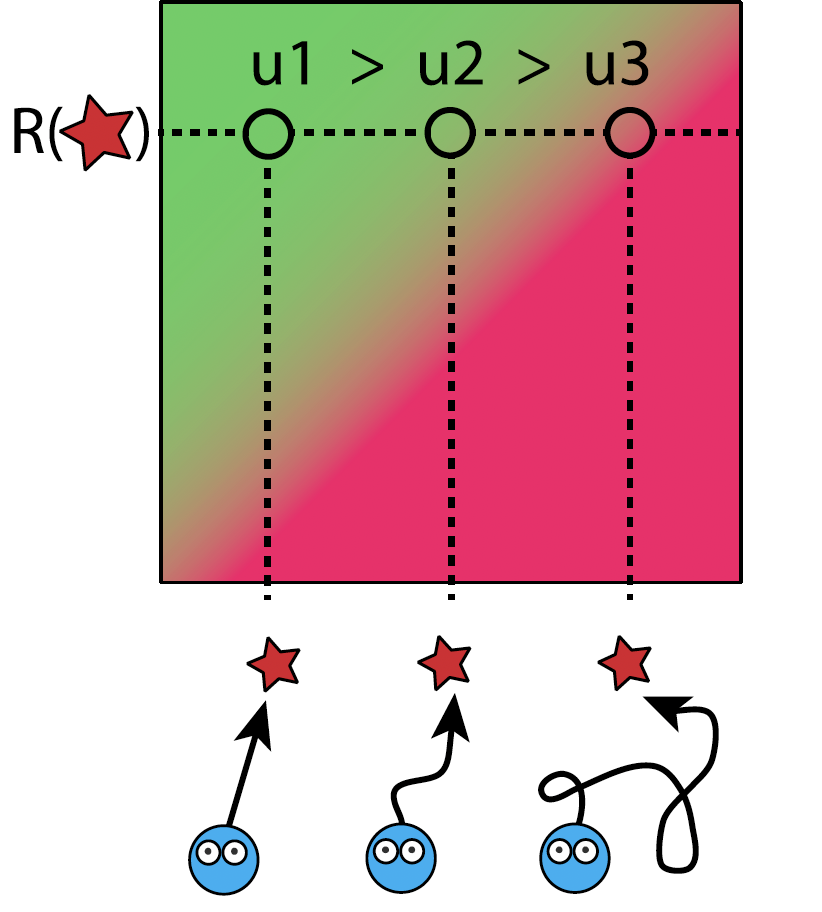
\includegraphics[width=0.3\textwidth]{utility2.png}
\end{center}
\vspace{0.3cm}
\begin{itemize}
    \item More efficient paths are less costly and therefore produce higher utilities
    \item When agents act, they will fulfill their goals as efficiently as possible to maximize utility
\end{itemize}
\end{frame}

\begin{frame}
\frametitle{Graded Preference Inference}
\begin{center}
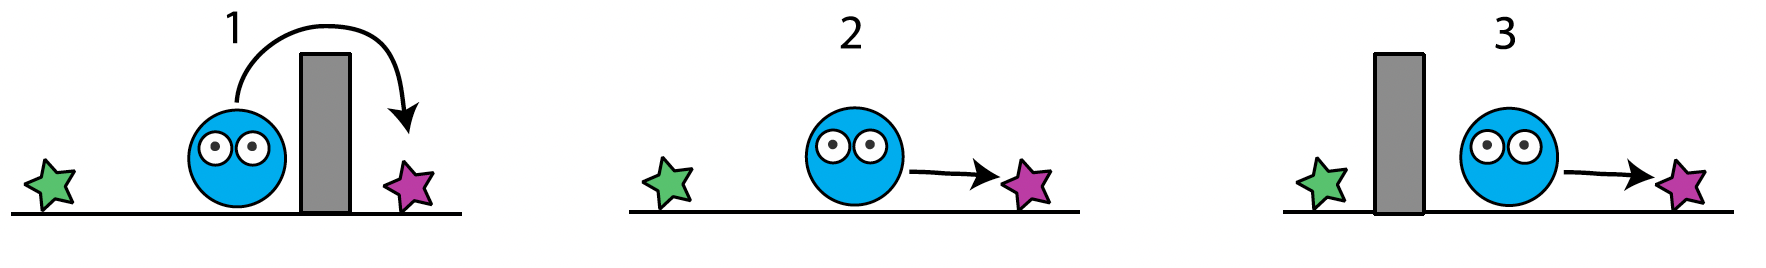
\includegraphics[width=0.7\textwidth]{utility3.png}
\end{center}

\vspace{0.3cm}
\begin{itemize}
    \item \textbf{Fig.1: Pursue high-cost}: Agent pays high cost (long detour) to get purple star → strong preference inference
    \pause
    \item \textbf{Fig.2: Pursue low-cost}: Agent pays low cost (short path) to get purple star → weak preference inference
    \pause
    \item \textbf{Fig.3: Forego high-cost}: Agent foregoes high cost (doesn't climb wall) to get green star, chooses purple instead → no preference inference
\end{itemize}
\end{frame}

\begin{frame}
\frametitle{Costs and Rewards Vary Across Agents}
\begin{center}
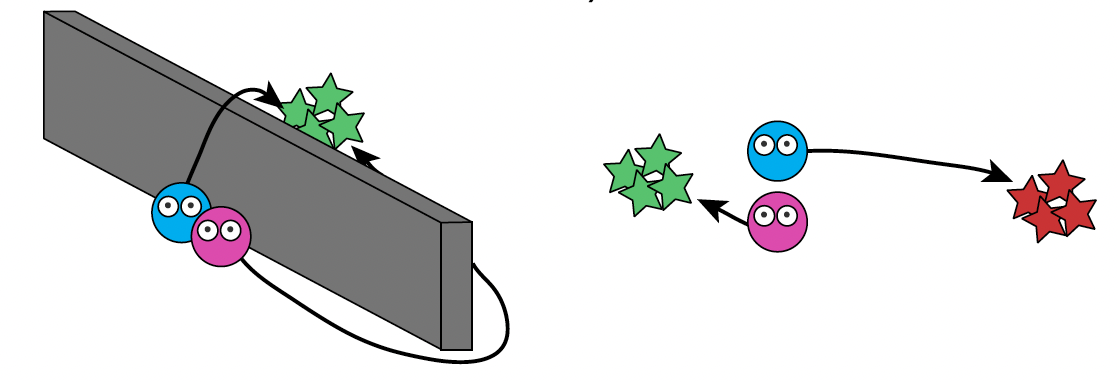
\includegraphics[width=0.7\textwidth]{utility4.png}
\end{center}

\vspace{0.3cm}
\begin{itemize}
    \item \textbf{Costs vary}: Blue agent can climb walls easily, pink agent cannot → different action costs
    \pause
    \item \textbf{Rewards vary}: Blue agent prefers red stars, pink agent prefers green stars → different goal values
    \pause
    \item \textbf{Same action, different inference}: Identical behavior can imply different preferences based on agent capabilities and values
\end{itemize}
\end{frame}

\section{Related Work}
\begin{frame}
\frametitle{Feature-Based Approach}
\begin{columns}
\begin{column}{0.5\textwidth}
\begin{center}
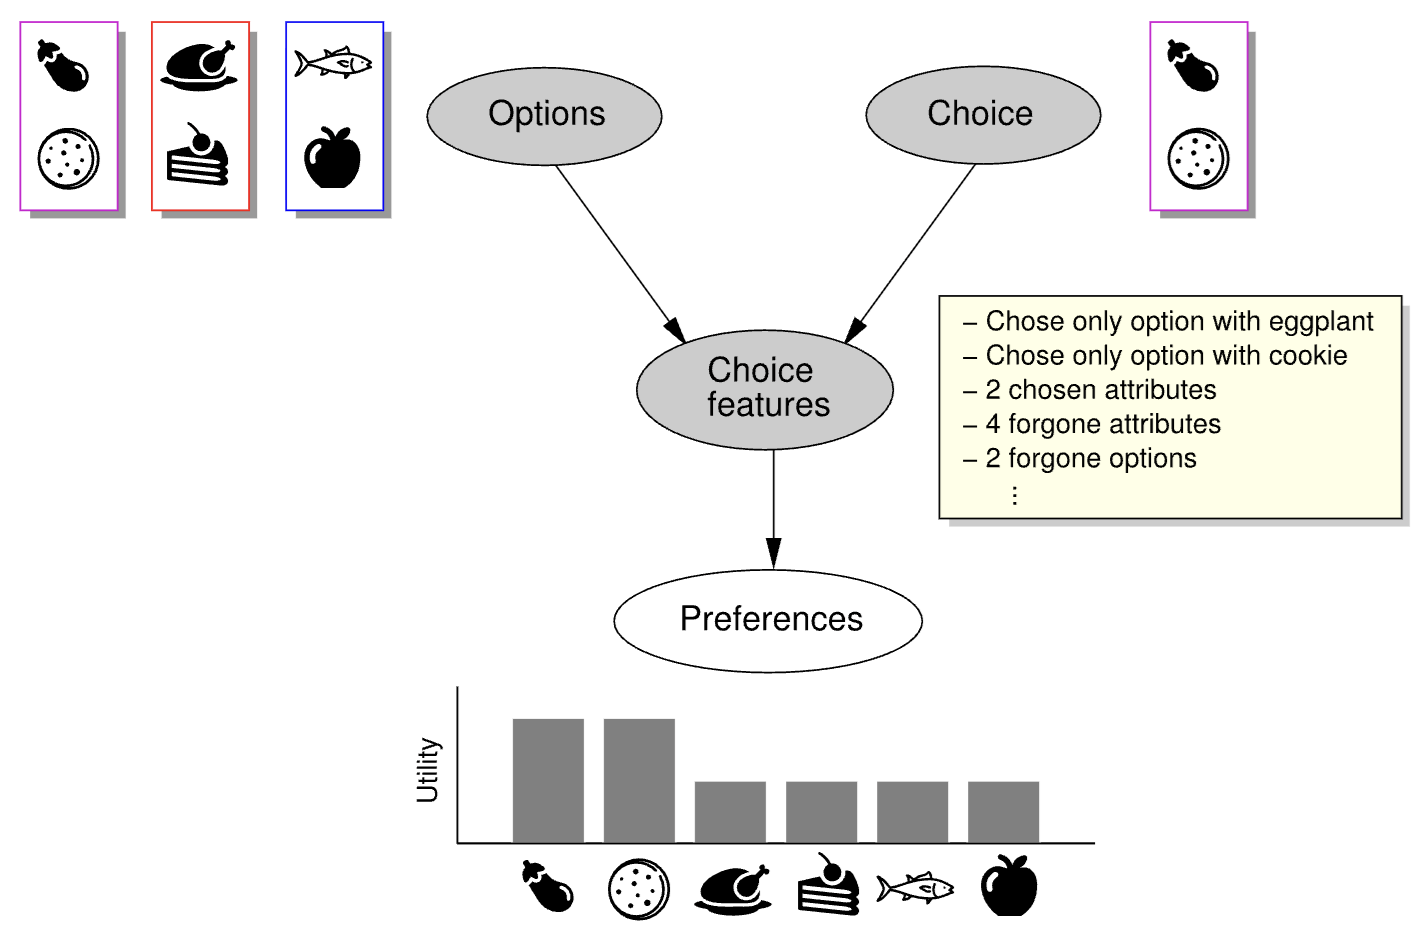
\includegraphics[width=0.95\textwidth]{feature_based.png}
\end{center}
\end{column}
\begin{column}{0.5\textwidth}
\begin{itemize}
    \item \textbf{Method}: Look at simple features of the choice and apply rules
    \item \textbf{Example}: Alice chooses \{eggplant sandwich\} over \{turkey, tuna, ham\}
    \item \textbf{Feature}: "She chose the only option with eggplant"
    \item \textbf{Rule}: "When someone picks the unique option, they probably like that thing"
    \item \textbf{Conclusion}: "Alice likes eggplant"
\end{itemize}
\end{column}
\end{columns}
\end{frame}

\begin{frame}
\frametitle{Inverse Decision-Making Approach}
\begin{columns}
\begin{column}{0.5\textwidth}
\begin{center}
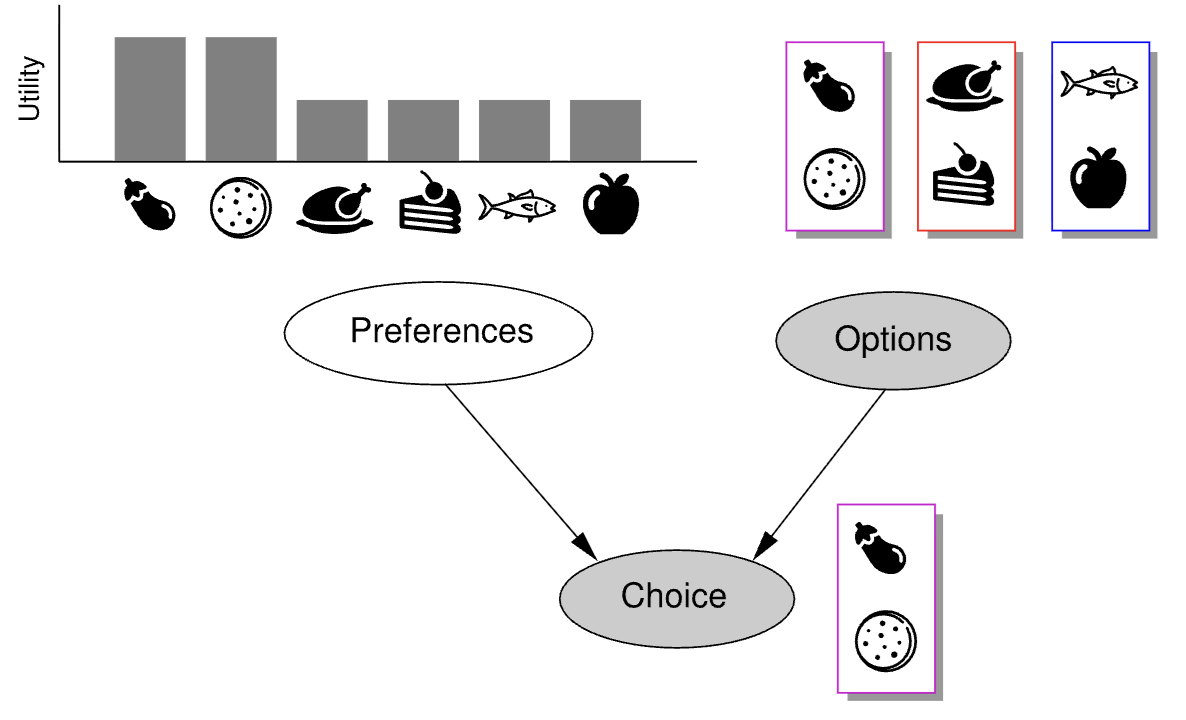
\includegraphics[width=0.95\textwidth]{inverse_decision.png}
\end{center}
\end{column}
\begin{column}{0.5\textwidth}
\begin{itemize}
    \item \textbf{Method}: Use a model of how people actually make decisions, then work backwards
    \item \textbf{Example}: Same choice - Alice chooses \{eggplant sandwich\} over \{turkey, tuna, ham\}
    \item \textbf{Model thinking}: "If Alice really liked eggplant, how likely would she be to make this choice? What if she liked turkey instead? What if she just wanted any sandwich?"
    \item \textbf{Calculation}: Uses math to figure out which preference scenario makes this choice most probable
    \item \textbf{Conclusion}: "Alice probably likes eggplant" (but with precise confidence levels)
\end{itemize}
\end{column}
\end{columns}
\end{frame}

\begin{frame}
\frametitle{NUC vs. Inverse Decision-Making}
\begin{itemize}
    \item \textbf{Similarity}: NUC is similar to inverse decision-making as it works on assumption that agents maximize utilities
    \item \textbf{Key Differences}:
    \begin{itemize}
        \item Uses events with complex spatiotemporal structures and not just isolated discrete choices
        \item Computes both variables costs and rewards, whereas inverse decision-making only infers rewards without costs
    \end{itemize}
\end{itemize}
\end{frame}

\begin{frame}
\frametitle{Inverse Planning}
\begin{columns}
\begin{column}{0.5\textwidth}
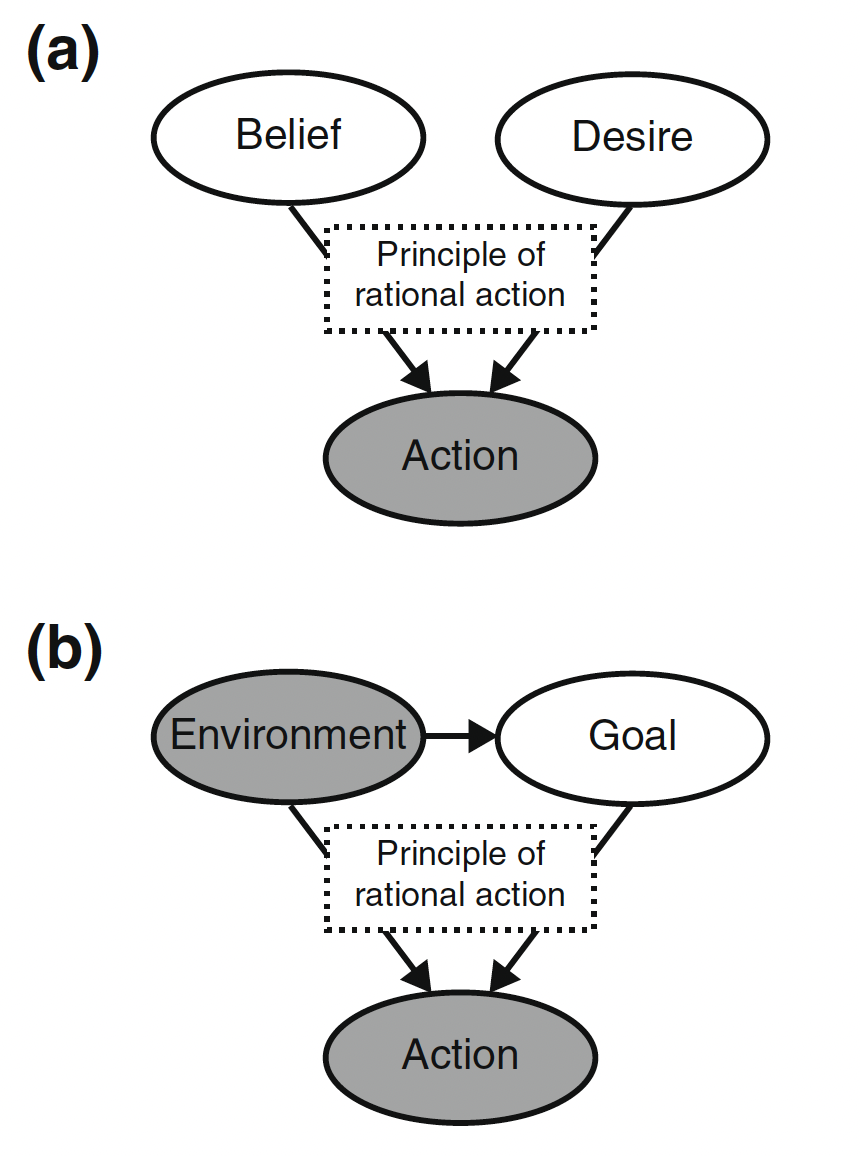
\includegraphics[width=1.0\textwidth]{inverse_planning.png}
\end{column}
\begin{column}{0.5\textwidth}
\textbf{Belief-Desire Psychology ("Forward-thinking")}
\begin{itemize}
    \item Belief + Desire → Action
    \item "Sarah believes store is open + wants coffee → walks to coffee shop"
\end{itemize}

\vspace{0.4cm}
\textbf{Inverse Planning ("Backward-thinking")}
\begin{itemize}
    \item Observe: Environment + Action → Infer: Goal
    \item "See maze layout + this path → agent wants point A"
\end{itemize}
\end{column}
\end{columns}
\end{frame}

\begin{frame}
\frametitle{Goal-Directed Action Understanding}
\begin{columns}
\begin{column}{0.5\textwidth}
\begin{center}
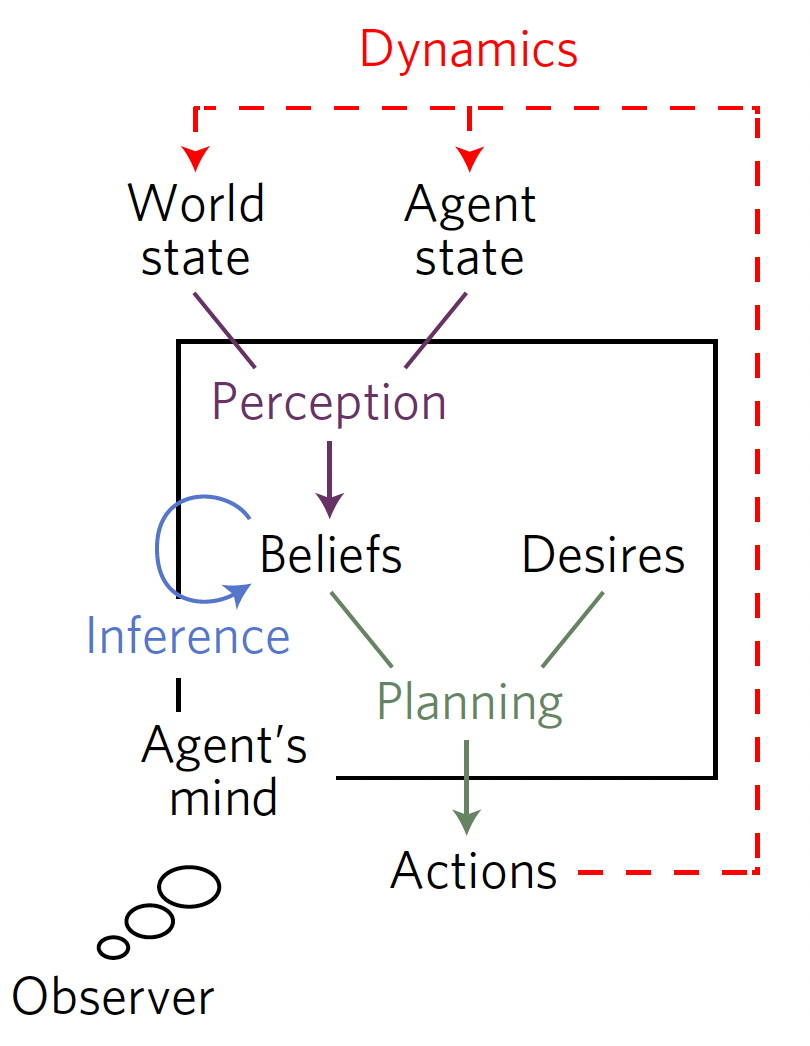
\includegraphics[width=0.95\textwidth]{goal_directed.png}
\end{center}
\end{column}
\begin{column}{0.5\textwidth}
\textbf{Limitations}
\begin{itemize}
    \item Model does not explain multiple causes behind other people's goals
    \item Treats cost as constant, observable and uniform across agents
\end{itemize}
\end{column}
\end{columns}
\end{frame}

\begin{frame}
\frametitle{Research Questions}
\begin{itemize}
    \item \textbf{RQ1}: Can NUC support joint inference of costs and rewards when we know neither, using a coherent generative model?
    \item \textbf{RQ2}: Does NUC drive fine-grained quantitative inferences or only coarse qualitative ones?
    \item \textbf{RQ3}: Is NUC a unified generative model supporting probabilistic inference, or a collection of simple heuristics?
\end{itemize}
\end{frame}

\section{NUC Computational Framework}

\begin{frame}
\frametitle{Hierarchical Mind Model}
\begin{center}
\begin{tabular}{|c|c|c|}
\hline
\textbf{Level} & \textbf{Component} & \textbf{Observable?} \\
\hline
4 & \textcolor{blue}{Desires} (Reward functions) & \textcolor{red}{No} \\
\hline
3 & \textcolor{blue}{Goals} (World states) & \textcolor{red}{No} \\
\hline
2 & \textcolor{blue}{Intentions} (Goal sequences) & \textcolor{red}{No} \\
\hline
1 & \textcolor{green}{Actions} (Behaviors) & \textcolor{green}{Yes} \\
\hline
\end{tabular}
\end{center}

\vspace{0.5cm}
\begin{center}
\Large $\downarrow$ \textbf{Inference Direction} $\uparrow$
\end{center}
\end{frame}

\begin{frame}
\frametitle{Generative Process}
\begin{center}
\begin{tabular}{c c}
\colorbox{blue!20}{\parbox{2.5cm}{\centering Desires \\ (Rewards)}} & \\
$\downarrow$ & + Costs \\
\colorbox{green!20}{\parbox{2.5cm}{\centering Goals}} & \\
$\downarrow$ & Utility Max \\
\colorbox{yellow!20}{\parbox{2.5cm}{\centering Intentions}} & \\
$\downarrow$ & Observable \\
\colorbox{red!20}{\parbox{2.5cm}{\centering Actions}} & \\
\end{tabular}
\end{center}
\end{frame}

\begin{frame}
\frametitle{MDP Planning per Goal}
\begin{center}
\textbf{Goal: Reach Object A}

\vspace{0.3cm}
$V^*(s) = \max_a \sum_{s'} P(s'|s,a)[R(a,s) - C(a,s) + \gamma V^*(s')]$

\vspace{0.5cm}
\textbf{Policy:} $p(a|s) \propto \exp(\sum_{s'} P(s'|s,a)V^*(s')/\alpha)$

\vspace{0.5cm}
Each goal $\rightarrow$ Separate MDP $\rightarrow$ Efficient path
\end{center}
\end{frame}

\begin{frame}
\frametitle{The Inference Problem}
\begin{center}
\begin{tabular}{c c c}
\colorbox{blue!20}{\parbox{2.5cm}{\centering \textbf{Hidden} \\ Costs \& Rewards}} 
& $\longrightarrow$ & 
\colorbox{red!20}{\parbox{2.5cm}{\centering \textbf{Observed} \\ Actions}} \\
& Forward & \\
& $\longleftarrow$ & \\
& \textcolor{red}{Bayesian Inference} & \\
\end{tabular}

\vspace{0.8cm}
$p(C,R|A) \propto p(A|C,R) \cdot p(C,R)$
\end{center}
\end{frame}

\begin{frame}
\frametitle{Two Types of Rationality}
\begin{center}
\begin{tabular}{|l|c|c|}
\hline
\textbf{Type} & \textbf{What} & \textbf{Formula} \\
\hline
Rational Choice & Intention selection & $p(I|C,R) \propto \exp(U(I)/\beta)$ \\
\hline
Rational Action & Efficient execution & $p(A|I)$ via MDP policy \\
\hline
\end{tabular}

\vspace{0.8cm}
\textbf{Likelihood:} $p(A|C,R) = \sum_I p(A|I) \cdot p(I|C,R)$
\end{center}
\end{frame}

\section{Experiments}
\begin{frame}
\frametitle{Experimental Setup}
\begin{itemize}
    \item \textbf{Domain}: Gridworld navigation tasks with agents moving toward goals
    \item \textbf{Participants}: Online studies using Amazon Mechanical Turk
    \item \textbf{Method}: Participants watch agent behaviors and make preference judgments
    \item \textbf{Key Variables}: Action costs (walls, detours), goal rewards (different objects), agent capabilities
    \item \textbf{Measures}: Preference strength ratings, choice predictions, confidence judgments
\end{itemize}
\end{frame}

\begin{frame}
\frametitle{Experiment 1: Graded Preference Inference}
\begin{itemize}
    \item \textbf{Question}: Do people make graded preference inferences based on action efficiency?
    \item \textbf{Design}: Agents choose between two goals with varying path costs
    \item \textbf{Manipulation}: High cost vs. low cost paths to preferred goal
    \item \textbf{Results}: 
    \begin{itemize}
        \item Higher costs → stronger preference inferences
        \item Lower costs → weaker preference inferences
        \item Linear relationship between cost and inferred preference strength
    \end{itemize}
    \item \textbf{Conclusion}: People make graded preference inferences consistent with NUC
\end{itemize}
\end{frame}

\begin{frame}
\frametitle{Experiment 2: Individual Differences in Costs}
\begin{itemize}
    \item \textbf{Question}: Do people consider individual differences in action costs?
    \item \textbf{Design}: Two agents with different capabilities (can/cannot climb walls)
    \item \textbf{Manipulation}: Same action, different costs for each agent
    \item \textbf{Results}:
    \begin{itemize}
        \item People adjusted preference inferences based on agent capabilities
        \item Wall-climbing agent: weaker preference for taking long route
        \item Non-climbing agent: stronger preference for taking long route
    \end{itemize}
    \item \textbf{Conclusion}: People consider individual cost differences when inferring preferences
\end{itemize}
\end{frame}

\begin{frame}
\frametitle{Experiment 5: Joint Cost-Reward Inference}
\begin{itemize}
    \item \textbf{Question}: Can people jointly infer costs and rewards from agent behavior?
    \item \textbf{Design}: Agents with unknown capabilities and unknown goal preferences
    \item \textbf{Manipulation}: Multiple trials revealing different cost-reward tradeoffs
    \item \textbf{Results}:
    \begin{itemize}
        \item People successfully inferred both costs and rewards simultaneously
        \item Judgments consistent with Bayesian model predictions
        \item Performance improved with more observations
    \end{itemize}
    \item \textbf{Conclusion}: NUC supports complex joint inference in realistic scenarios
\end{itemize}
\end{frame}

\section{Discussion}
\begin{frame}
\frametitle{Discussion}
\begin{itemize}
    \item \textbf{Key Findings}: People use Naive Utility Calculus for preference inference
    \begin{itemize}
        \item Make graded inferences based on action efficiency
        \item Consider individual differences in costs and rewards
        \item Perform complex joint inference of multiple variables
    \end{itemize}
    \item \textbf{Theoretical Contribution}: NUC as a unified computational framework
    \begin{itemize}
        \item Goes beyond simple heuristics
        \item Supports probabilistic inference mechanisms
        \item Handles spatiotemporal action sequences
    \end{itemize}
    \item \textbf{Future Directions}: 
    \begin{itemize}
        \item Real-world applications beyond gridworlds
        \item Neural mechanisms underlying utility-based reasoning
        \item Cross-cultural and developmental studies
    \end{itemize}
\end{itemize}
\end{frame}

\end{document}